\subsection{Algoritmos de ordenamiento}

En la Figura~\ref{fig:sort_complejidad} se observa el tiempo de ejecución promedio de cada algoritmo en función del tamaño del arreglo, junto con líneas de referencia teóricas. Los cuatro algoritmos siguen razonablemente bien una tendencia $O(n \log n)$ en la escala logaritmica utilizada, incluyendo Quick Sort, para el cual se utilizó una elección de pivote aleatorio para mejorar su rendimiento. Las pequeñas desviaciones respecto a la curva teórica en cada algoritmo se explican por factores constantes propios de cada implementación asi como diferencias en como los algoritmos afrontan distintas entradas, factores que la notación asintótica no captura, pero que sí afectan el tiempo real de ejecución. \\

\begin{figure}[H]
    \centering
    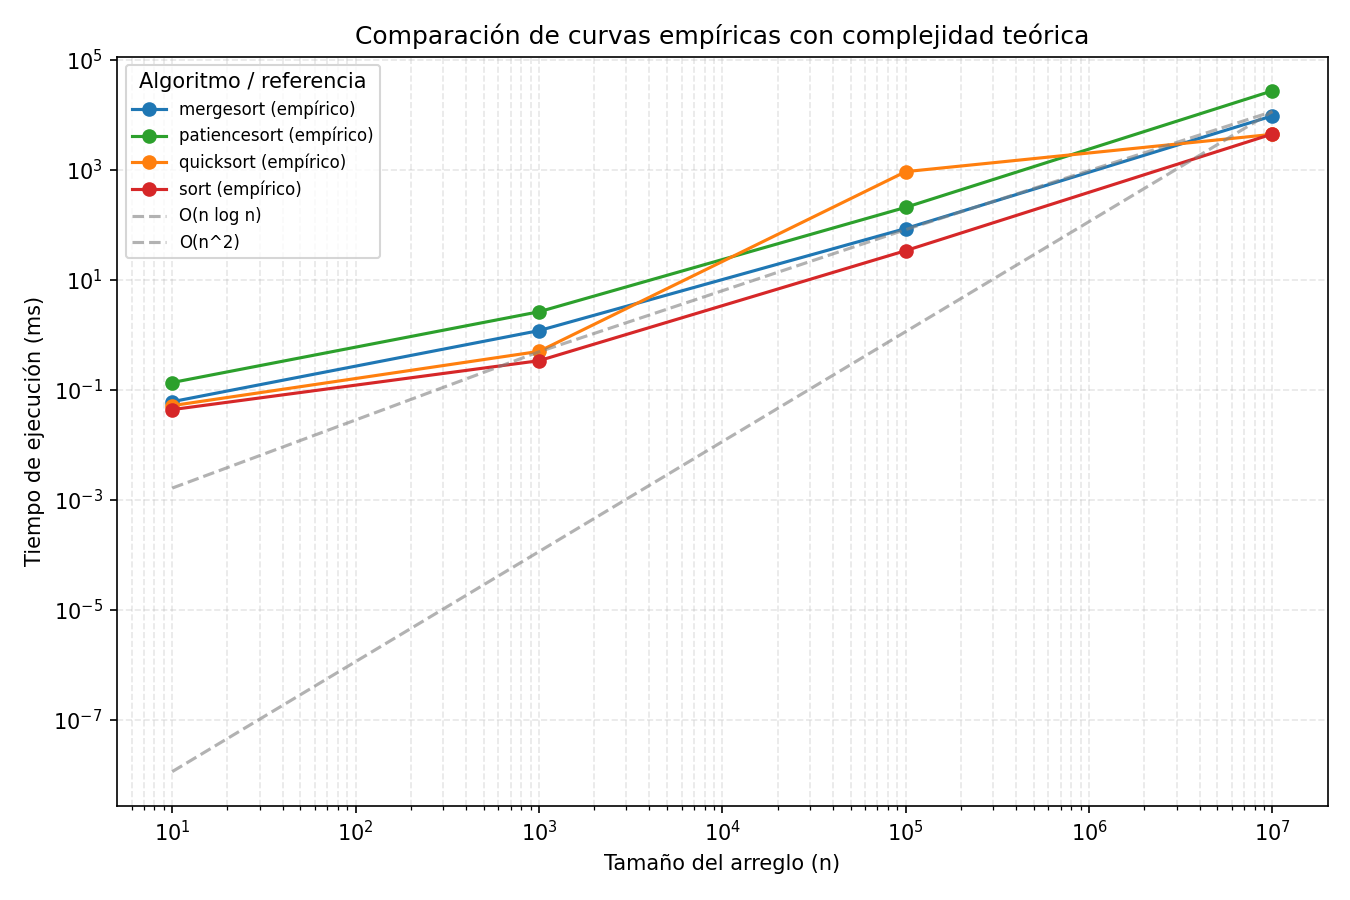
\includegraphics[width=0.6\textwidth]{complejidad_teorica.png}
    \caption{Tamaño del arreglo con respecto al tiempo de ejecución promedio de los casos de prueba. Separado por algoritmo y con complejidad teórica como referencia.}
    \label{fig:sort_complejidad}
\end{figure}

La Figura~\ref{fig:sort_memoria} muestra la memoria auxiliar utilizada por cada algoritmo respecto al tamaño del arreglo. Se observa una clara diferencia según si el algoritmo ordena \textit{in-place} o no: Quick Sort y \texttt{std::sort} ambos in-place, sin necesidad de estructuras auxiliares en el heap más allá de la pila de recursión muestran un uso de memoria prácticamente nulo y constante, independiente del tamaño de entrada, lo cual coincide con su complejidad de espacio auxiliar $O(\log n)$ (memoria de pila, no medida por este mecanismo basado en el heap). En contraste, Merge Sort y Patience Sort sí requieren memoria auxiliar proporcional a $n$: Merge Sort porque su función de fusión crea explícitamente vectores temporales para combinar las mitades ordenadas, y Patience Sort porque debe mantener simultáneamente todos los montones (\textit{piles}) generados durante el proceso de inserción. Patience Sort exhibe un uso de memoria notablemente mayor que Merge Sort para un mismo $n$, lo que se explica por el peor caso estructural del algoritmo: en arreglos ascendentes, cada nuevo elemento es mayor o igual al tope de todos los montones existentes, forzando la creación de un montón nuevo por cada elemento procesado, en vez de reutilizar montones existentes.

\begin{figure}[H]
    \centering
    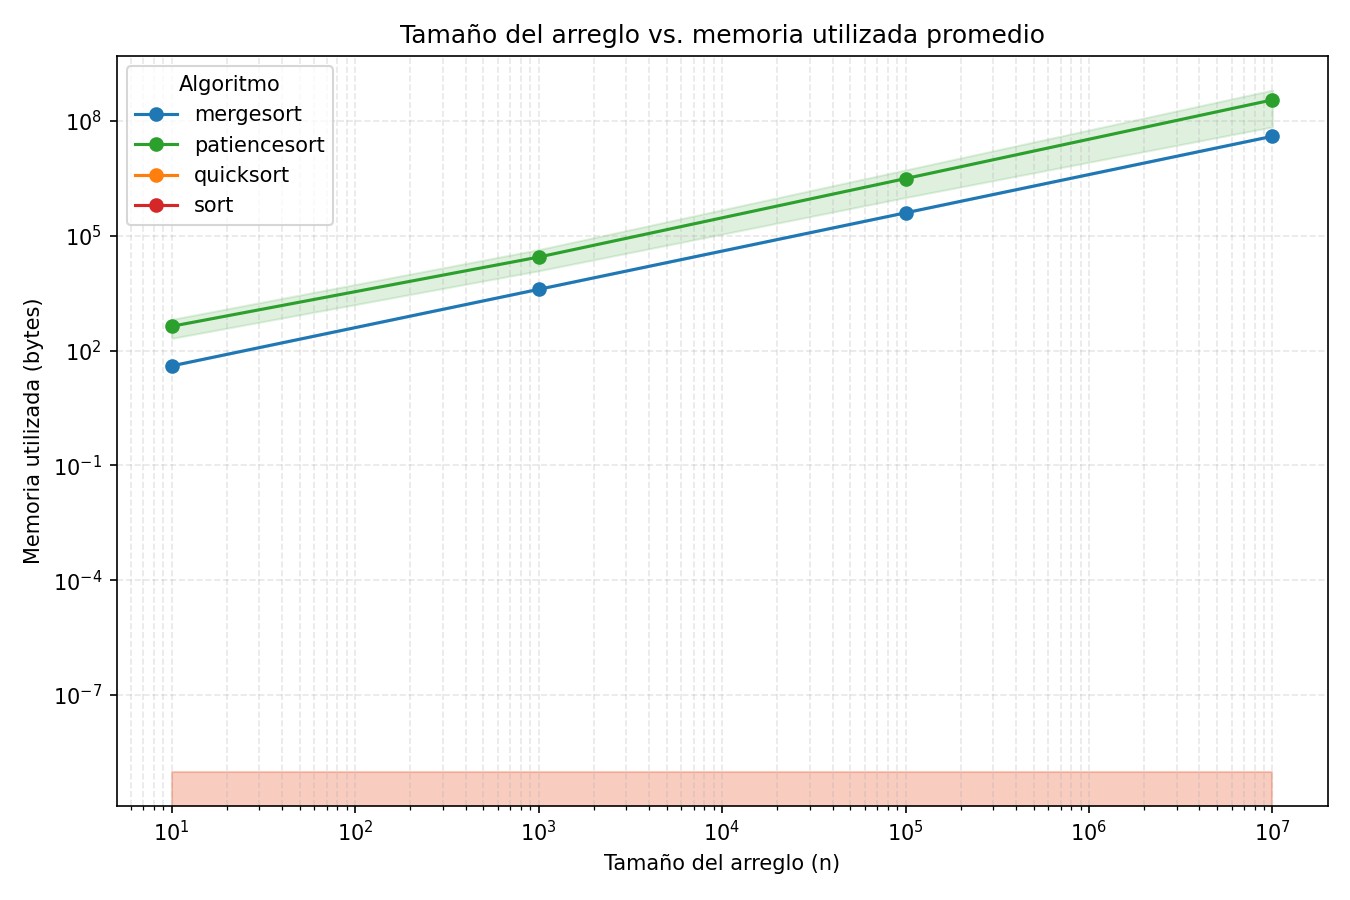
\includegraphics[width=0.7\textwidth]{tamano_vs_memoria.png}
    \caption{Tamaño del arreglo con respecto a la memoria utilizada promedio de los casos de prueba. Separado por algoritmo.}
    \label{fig:sort_memoria}
\end{figure}

Finalmente, la Figura~\ref{fig:sort_dominio} compara el tiempo de ejecución promedio de cada algoritmo entre los dominios D1 y D7. Patience Sort es consistentemente el algoritmo más lento de los cuatro, coherente con el mayor overhead de gestión de montones descrito anteriormente. 



\begin{figure}[H]
    \centering
    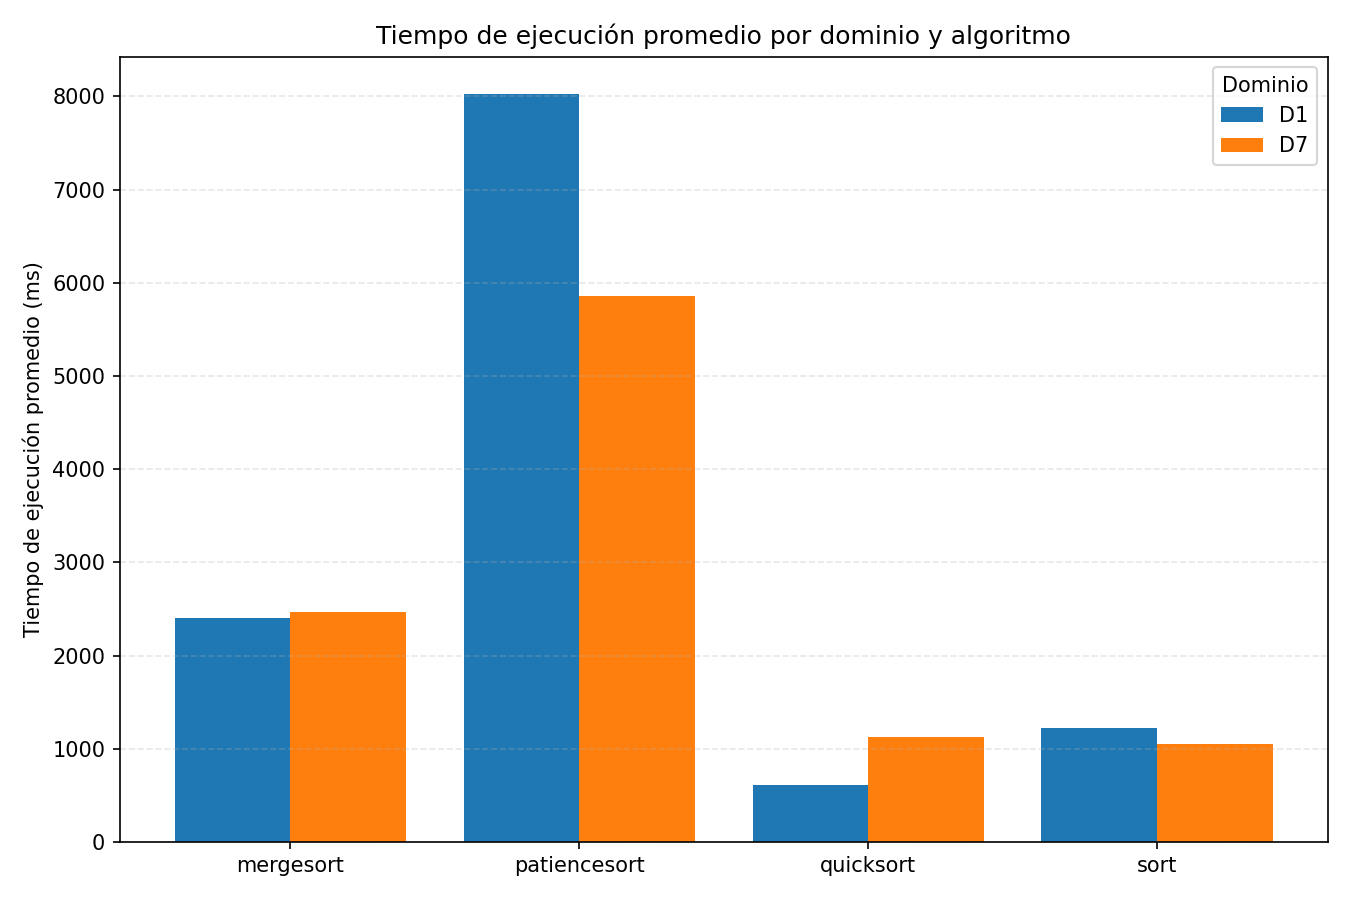
\includegraphics[width=0.6\textwidth]{tiempo_por_dominio.png}
    \caption{Tiempo de ejecución promedio de cada uno de los algoritmos en los dominios D1 y D7.}
    \label{fig:sort_dominio}
\end{figure}


\subsection{Algoritmos de Multiplicación de Matrices}

En cuanto a los algoritmos de multiplicación de matrices, la Figura~\ref{fig:matrix_complejidad}
muestra que tanto el algoritmo naive como Strassen siguen de cerca sus
complejidades teóricas esperadas, $O(n^3)$ y $O(n^{2.807})$ respectivamente, en el
rango de tamaños evaluado. Esto confirma que ambas implementaciones se comportan
según lo predicho por el análisis asintótico, sin degradaciones inesperadas
atribuibles a errores de implementación.

\begin{figure}[H]
    \centering
    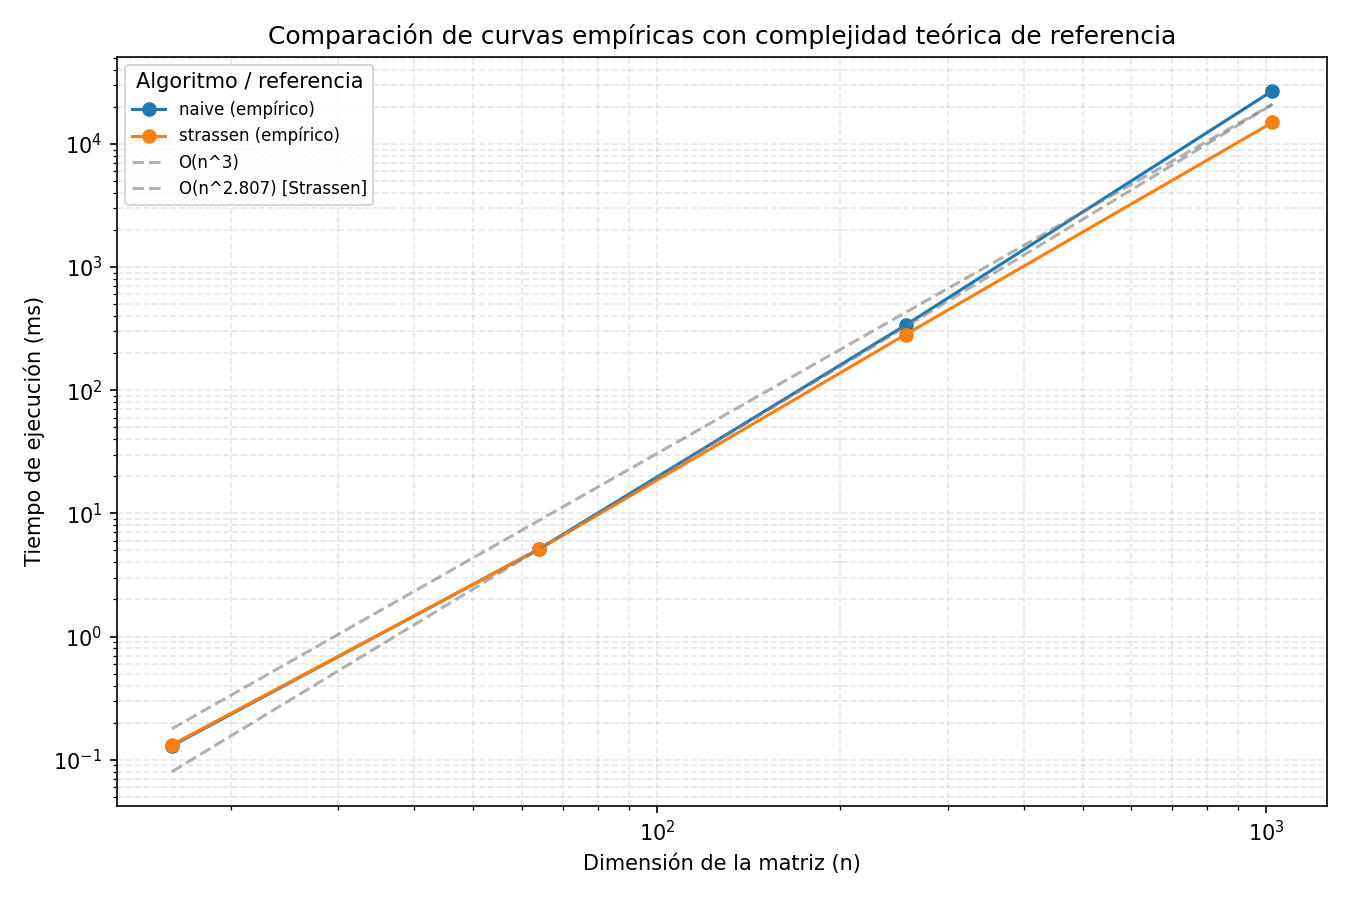
\includegraphics[width=0.6\textwidth]{m_complejidad_teorica.png}
    \caption{Tamaño de la matriz con respecto al tiempo de ejecución promedio de los casos de prueba. Separado por algoritmo y con complejidad teórica como referencia.}
    \label{fig:matrix_complejidad}
\end{figure}

La Figura~\ref{fig:matrix_memoria} muestra la memoria auxiliar utilizada por cada algoritmo en función de la dimensión de la matriz. Para tamaños pequeños, ambos
algoritmos utilizan una cantidad de memoria similar, ya que Strassen, por debajo de su umbral de caso base, delega directamente en una multiplicación equivalente a la naive sin recurrir a el costo adicional de la recursión. Sin embargo, a partir de cierto tamaño la memoria utilizada por Strassen crece notablemente por sobre la de naive. Esto se explica por la naturaleza recursiva del algoritmo que por cada nivel de la recursión, crea multiples submatrices utilizando memoria adicional. 

\begin{figure}[H]
    \centering
    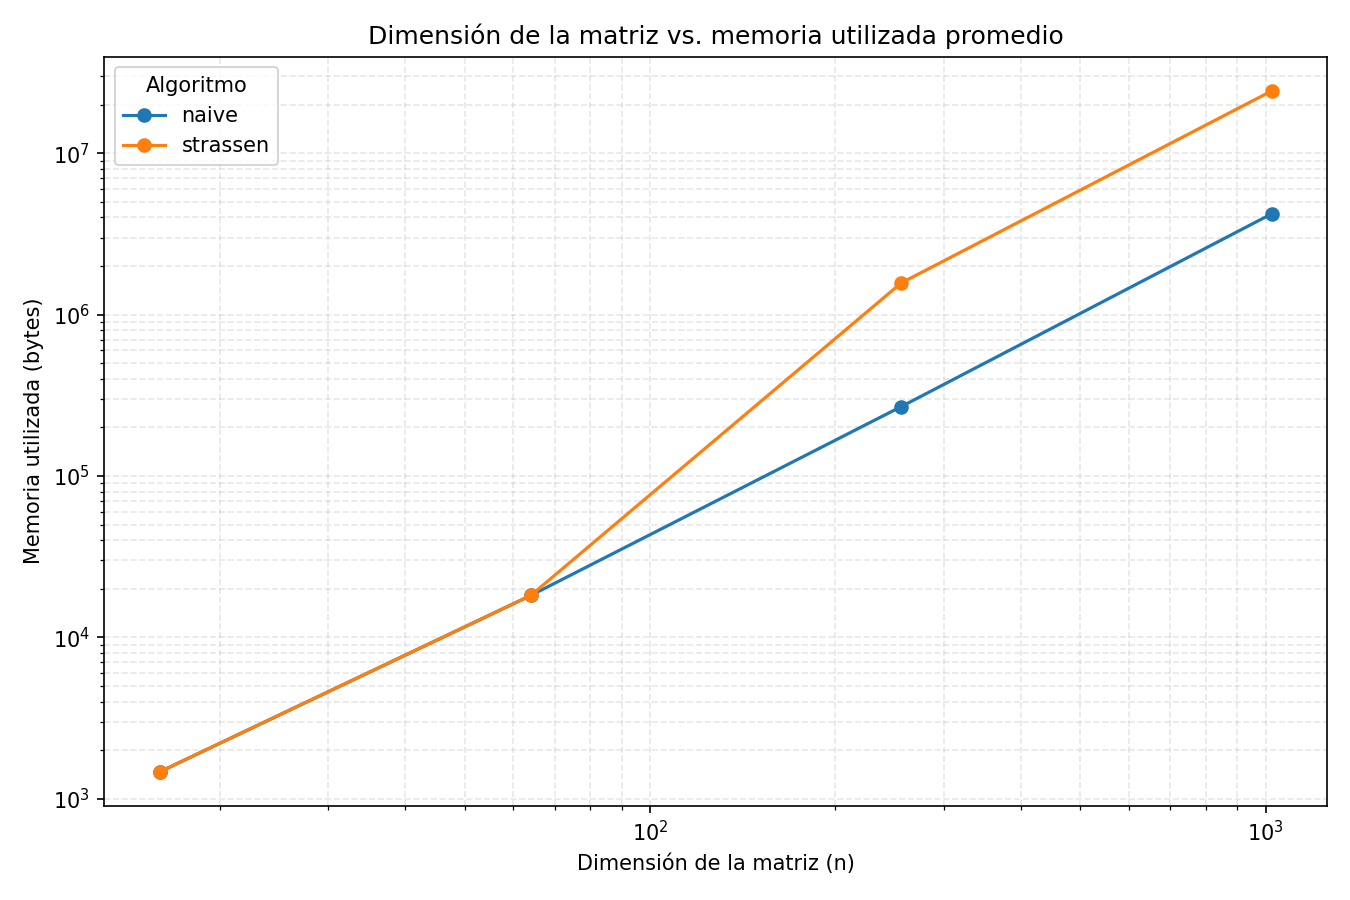
\includegraphics[width=0.6\textwidth]{m_tamano_vs_memoria.png}
    \caption{Tamaño de la matriz con respecto a la memoria utilizada promedio de los casos de prueba. Separado por algoritmo.}
    \label{fig:matrix_memoria}
\end{figure}

Por último, la Figura~\ref{fig:matrix_dominio} compara el tiempo de ejecución promedio de ambos algoritmos entre los dominios D0 (\{0,1\}) y D10 (\{0,\dots,9\}). \\
Strassen es notablemente más rápido que naive en ambos dominios, lo que resulta coherente con la Figura~\ref{fig:matrix_complejidad} y con la ventaja asintótica de Strassen para matrices de mayor tamaño. Además, Strassen muestra un tiempo de ejecución prácticamente idéntico entre D0 y D10, lo cualconcuerda con lo esperado. Tanto naive como Strassen realizan exactamente las mismas operaciones aritméticas sin importar los valores concretos de los coeficientes de la matriz, por lo que el dominio de valores no debería afectar el tiempo de ejecución de ninguno de los dos algoritmos, a diferencia de lo observado en algunos algoritmos de ordenamiento donde la cantidad de valores duplicados sí incide en el número de comparaciones
realizadas.

\begin{figure}[H]
    \centering
    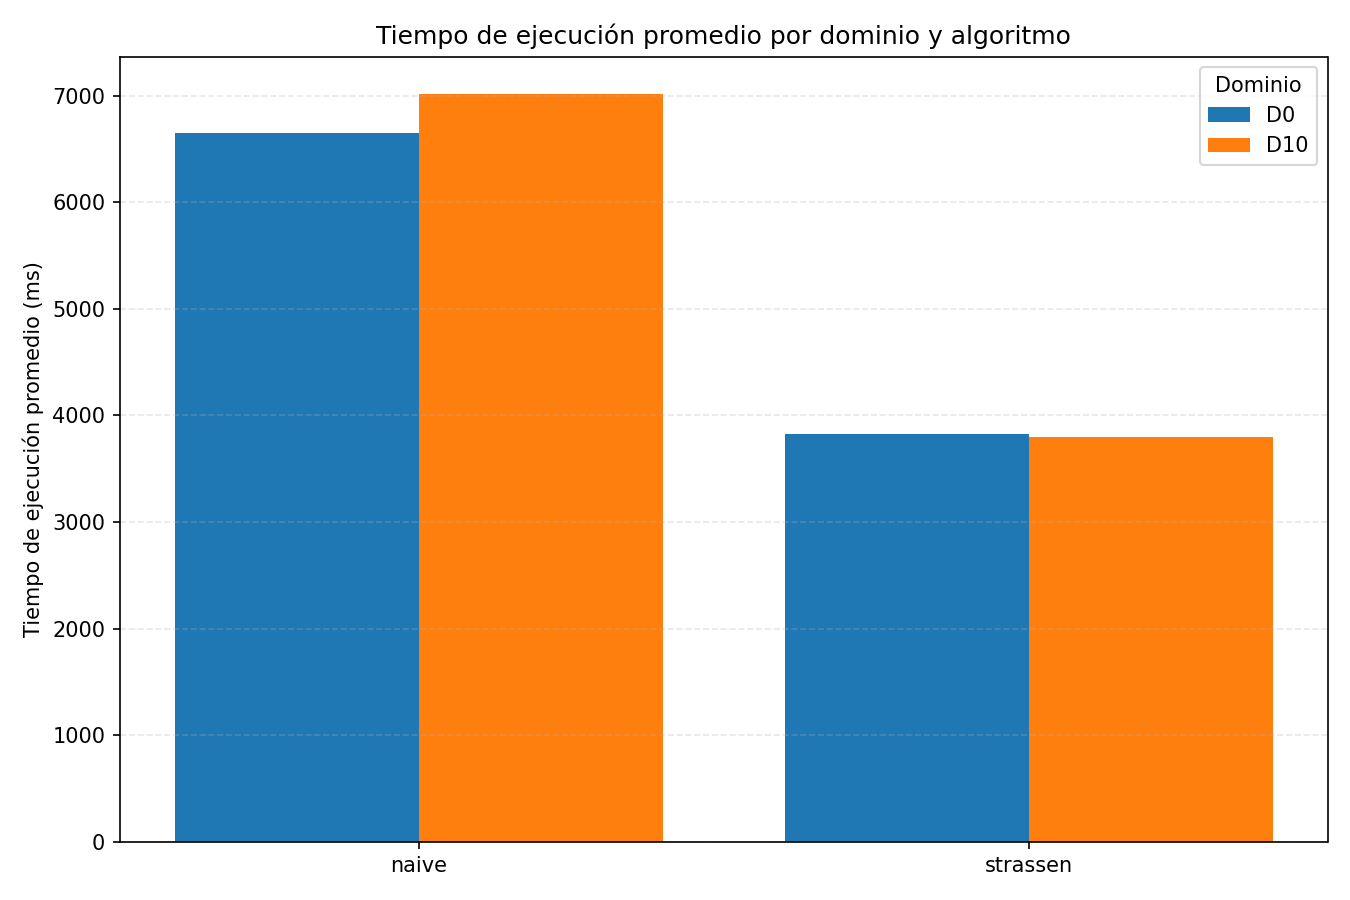
\includegraphics[width=0.6\textwidth]{m_tiempo_por_dominio.png}
    \caption{Tiempo de ejecución promedio de cada uno de los algoritmos en los dominios D0 y D10.}
    \label{fig:matrix_dominio}
\end{figure}
